\documentclass[10pt,a4paper]{article}
\usepackage[utf8]{inputenc}
\renewcommand{\familydefault}{\sfdefault}
\usepackage{amsmath,amssymb,sansmathfonts,color,graphicx,afterpage,mathtools,bm,hyperref,listings,subcaption}
\graphicspath{{figures/}}
\usepackage[margin=2cm]{geometry}
\setlength{\parskip}{3pt}
\allowdisplaybreaks
\lstset{language=C++, basicstyle=\ttfamily}
\mathtoolsset{showonlyrefs}

\newenvironment{code}
{\newline
\hspace*{1cm} \begin{minipage}{\textwidth} \vspace*{0.2cm} \textrm}
{\vspace*{0.2cm}\end{minipage}}
\newcommand{\carrow}{-\textgreater}
\newcommand{\arrow}{$\rightarrow$ }

\title{\textbf{Control Theory -- Assignments}}
\date{\vspace{-5ex}}

\begin{document}

\maketitle

\section{Introduction}
The examination of the course Control Theory is based on practical assignments in which you will apply several techniques taught during the course in order to control the cart presented in Figure \ref{fig:cart}. This cart has two separately driven wheels in the front and can be equipped with a free axis with two wheels in the back for moving on a straight line, or with a swivel wheel when rotation is required. It is controlled by an Arduino Mega, running MicroOS as software framework. For more information on this system, you are referred to the tutorial session.

For these assignments you work in groups of 2 students. If your cart has a swivel wheel, you must perform assignments 1, 2, and 4. Students with a 4-wheeled cart perform assignments 1, 2, and 3. Put your results in a slideshow which is understandable on its own. The deadline of handing in this slideshow will be announced on Toledo. Later you will be invited to defend your work orally. \textit{You are allowed to change one of the assignments by an own invented \underline{challenging} exercise performed on the cart. First discuss your assignment with the teaching assistants.}

In case there are questions, we strongly suggest to consult your fellow students about the matter. Discuss amongst yourselves and try to come up with the answer. In case you cannot get to a consensus, you can ask the teaching assistants of the course to help you out. They will be available for questions \textbf{during office hours only (announced on Toledo)}. Keep in mind that this assignment acts as your examination and an excessive amount of questions might be penalized in the end. Therefore think before you consult the teaching assistants. The one big exception is of course a broken cart. Don't hesitate to pass by so that we can fix whatever is broken.

\begin{figure}
  \centering
  \begin{subfigure}[c]{0.46\columnwidth}
    \centering
    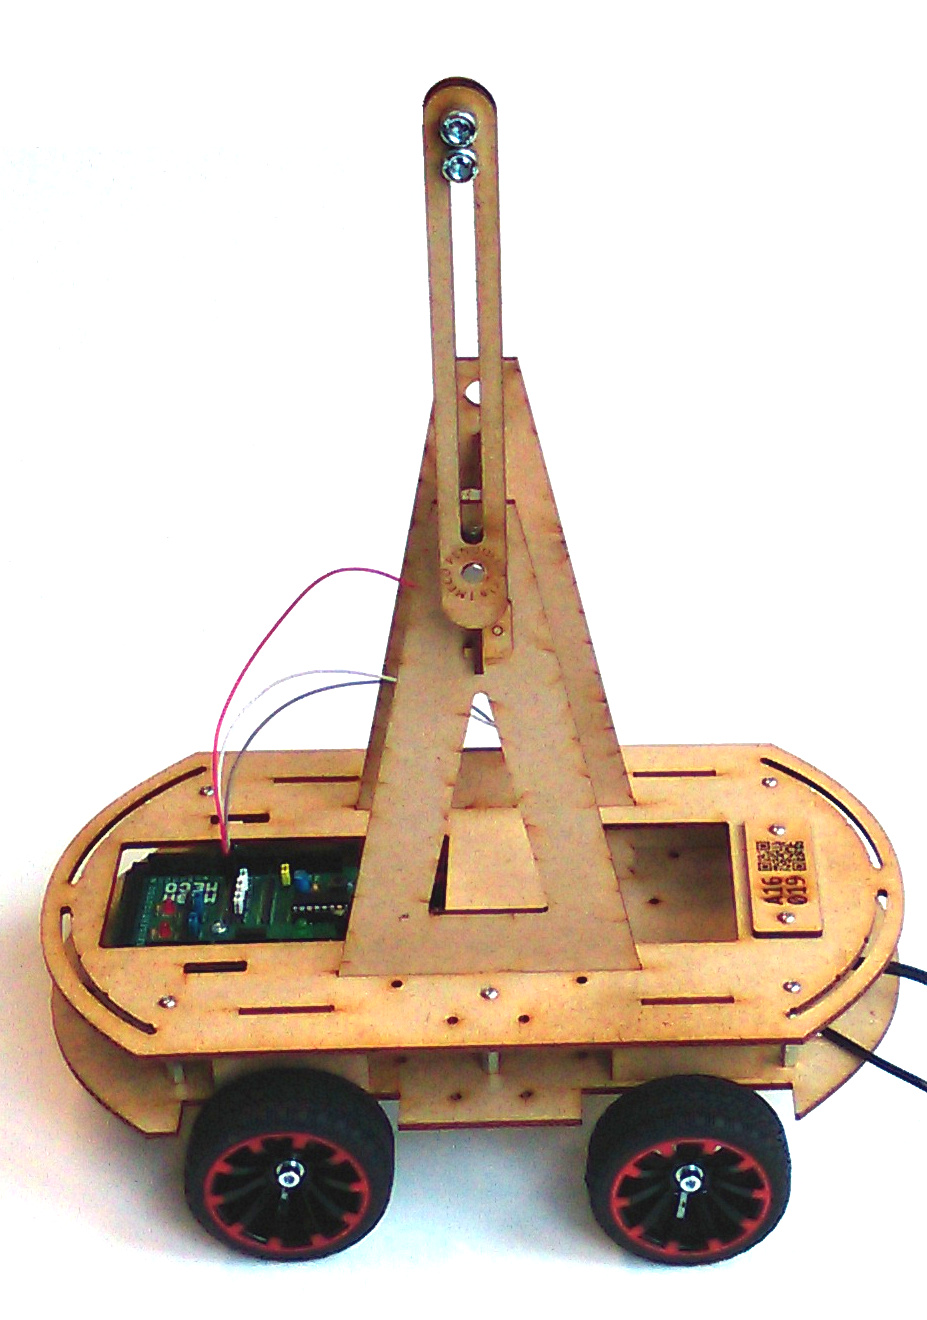
\includegraphics[scale=0.1]{figures/pendulum.jpg}
    \caption{4-wheeled cart with pendulum}
  \end{subfigure}
  \begin{subfigure}[c]{0.46\columnwidth}
    \centering
    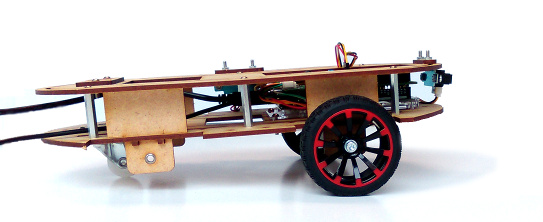
\includegraphics[scale=0.4]{figures/swivel.jpg}
    \caption{Cart with swivel wheel}
  \end{subfigure}
\caption{Setup used during the assignments.}
\label{fig:cart}
\end{figure}


\section{How to make us happy?}
Below, you find a (non-exhaustive) list of suggestions what to put in your final presentation. For each slide, think about what you want to achieve with it: should it reflect your controller design, should it show the result of an experiment, do you want to compare the theoretical model with the identification, ... Secondly, think about which figures and equations will be most informative. For example: showing the error signal is usually more informative than showing the reference and the output together. Make sure your slides reflect the assignment: stick to the titles and divisions as mentioned in the assignment.

\subsection{Identification}
\begin{itemize}
\item Derive the theoretical model. What are the inputs, outputs and states? What are their fysical units?
\item What excitation do you apply and why?
\item Compare the identified model with a fysical model. What are the differences and can you explain them?
\item What can you tell about linearity of the system. Can you identify some non-linearities?
\end{itemize}

\subsection{Control}
\begin{itemize}
\item Motivate why you choose a specific type of controller: PI, lead, PID, lag, ...
\item Always show Bode diagrams relevant to your design and interpret them. Open loop, closed loop, ...
\item Write down the transfer function of your controller along with some Bode plot.
\item Write down the recursive formulation of the controller, as implemented on the Arduino.
\item Show relevant input and output signals such as the tracking error, the control input (check for saturation!), the output, the reference, ...
\item Compare your experiment with a simulation. Can you explain the differences?
\end{itemize}

\section{Assignments}

\subsection{Assignment 1: velocity control of the cart}
In this exercise you will design a velocity controller for the two motors such that they can track a desired velocity setpoint. In order to accomplish this, perform the following steps:
\paragraph{Step 1: Identification of the motor(s)} The goal of this step is to find an appropriate model for the motors. \textit{Perform and document all steps necessary to identify the motors. Validate the acquired model by observing the response for given input trajectories for both the theoretical model and the real system. Can you explain certain deviations?}
\paragraph{Step 2: Design a velocity controller} Once you obtain a model of the motors, you can design a velocity controller in order to track a velocity setpoint for a motor. You should design a controller with zero steady-state error using frequency response methods. \textit{What type of controller do you choose? Show all steps and choices during the design procedure. Show all relevant Bode diagrams. Implement the controller on the Arduino and compare the behavior to simulations}.
\paragraph{Step 3: Velocity control of the cart} Since you can control both motors of the cart, you can combine this to control the velocity of the cart driving on a straight line. \textit{How do your controllers from step 2 perform for controlling the whole cart? Find a way of applying a constant force disturbance to the cart. Is your controller still following the velocity setpoint (both in theory and practice)? If not, adapt your controller such that the cart reaches its desired velocity}.

\subsection{Assignment 2: position control of the cart}
You can now start controlling the cart's position. The motors are considered to be velocity driven, so you should keep the previously designed velocity controllers in place, as you will be putting another loop around them.
\paragraph{Step 1: Modeling the plant} In order to design a decent controller, you again need a model of the system. The position controller provides a new setpoint to the speed controller. As the tracking is not perfect ($v_{ref}\left(t\right) \neq v\left(t\right)$), the closed loop dynamics should be included in the model of the system. \textit{Make a block diagram of the overall position control system. Where does the speed loop appear? What is the consequence of the speed loop's limited bandwidth? Show the latter on an open-loop bode diagram.}
\paragraph{Step 2: Proportional control} In combination with the speed loop, a proportional position controller will already do a good job. \textit{Design a proportional controller for the positioning system, based on its root-locus. Implement the controller on the platform and show some relevant plots. Is the influence of the non-ideal speed controller visible in the root-locus and how? What other controller would you use to improve performance? Show the improvement with relevant figures, both in theory and in practice.}
\paragraph{Step 3: Position sensor fusion} Apart from the encoders, the front distance sensor also provide a read of the position. These can be combined to obtain a better estimate of the absolute position w.r.t. some wall. We propose a model with two states: $d$, the initial distance to the wall when the encoders read 0, and $s$, the relative distance the car has traveled. The discrete time dynamics become:
\begin{equation}
\begin{bmatrix} d\\s \end{bmatrix}_{k+1} = \begin{bmatrix}1&0\\0&1\end{bmatrix}\begin{bmatrix} d\\s \end{bmatrix}_{k} + \begin{bmatrix}0\\T_s\end{bmatrix}v_k
\end{equation}
\textit{Write down the measurement equations for this system. Make a state estimator for the proposed model and validate the estimation process. What happens if the measurements become inconsistent? Device an experiment to demonstrate your findings.}

\subsection{Assignment 3: control of an inverted pendulum attached to the cart}
In this part, the cart will be used to control an inverted pendulum. By measuring the pendulum's angle, the open-loop unstable system can be rendered stable. Make sure to get a 4-wheeled cart as you won't benefit from a swivel wheel in the back. In order to get a good controller, we propose the following steps:
\paragraph{Step 1: Deriving the model} In order to design a controller, one has to acquire a model. Since the system is unstable, simple identification techniques are inapplicable. Therefore, you must resort to a theoretical model of the system. Since you already have velocity control on the cart, you can consider speed to be the input of the system. \textit{Derive a theoretical non-linear model for the velocity-driven inverted pendulum. Next, linearize the model in the neighborhood of the stable and unstable equilibrium position, i.e. the bottom and top position. Measure the pendulum's natural frequency and use it to estimate the parameters of the stable and unstable model. What are the poles of the two models?}
\paragraph{Step 2: Obtaining a discrete state-space model} Since we are implementing a controller for an unstable system, pole placement seems like a good solution\footnote{Frequency domain controller design is of course still applicable but stability conditions are a bit more tricky. In that regard, state-space is more hakuna matata.}. As the controller will be running on a digital platform, you need a discrete time model to design a discrete time controller. \textit{Derive a state-space description from the linearized theoretical model (Hint: you need exactly 3 states of which one is the cart position). Perform a discretization on the state-space to obtain a discrete time equivalent. How do the discrete time states relate to the original states?}
\paragraph{Step 3: Controller design} Based on the theoretical model, we should be able to design a state estimator and state-feedback gain. A pole-placement approach will (in this case) works best, if the poles of the controller are located at conservative locations, e.g. 1 rad/s. If this design succeeds, you can try to push the bandwidth of the controller further. \textit{Compute a state-feedback gain and a state estimator with appropriate pole locations. Implement your controller on the platform and do some relevant experiments. Try to push the bandwidth as far as possible. What do you see as the bandwidth increases? Validate your findings experimentally.}
\paragraph{Step 4: Imperfect angle calibration} \textit{What happens if the sensor's zero value is erronously calibrated, i.e. the sensor's zero position does not correspond to the pendulum's equilibrium position? Show via simulation what happens and try to experimentally validate it. Can you explain this behavior? Try to resolve this issue (Hint: integral feedback should do the trick) and implement your new controller.}

\subsection{Assignment 4: estimation and control of a two-wheel driven cart}
This assignment considers the cart mounted with the swivel wheel and with two infrared sensors. Because the cart has two separately driven wheels, it acts as a two-wheel drive (2WD) system that can move in the horizontal plane.
The system under consideration is shown in Figure \ref{fig:cartkalman}. The 2WD cart moves around in the world's $XY$ plane. The coordinates of the cart's (geometric) center point are denoted by $(x_{\mathrm{c}},y_{\mathrm{c}})$, and $\theta$, the angle between the $X$-axis and the cart's longitudinal axis, determines the cart's orientation. A local coordinate system $X'Y'$ is attached to the cart at its center. The goal of this assignment is to estimate the cart's position and orientation $(x_{\mathrm{c}},y_{\mathrm{c}},\theta_{\mathrm{ref}})$ by means of a Kalman filter and to use this estimate to make the cart follow a reference trajectory specified in terms of $(x_{\mathrm{c,ref}},y_{\mathrm{c,ref}},\theta_{\mathrm{ref}})$.

This assignment uses the velocity controller, designed in Assignment 1, and assumes that it is perfect. That is, the actual velocities of the left and right wheel, denoted by $\omega_{\mathrm{L}}$ [rad/s] and $\omega_{\mathrm{R}}$ [rad/s], correspond to their desired values $\omega_{\mathrm{L,des}}$ [rad/s] and $\omega_{\mathrm{R,des}}$ [rad/s].
To locate itself with respect to nearby objects, the cart is able to take distance measurements from two infrared sensors: one frontal, and one lateral (one side only).
Without infrared measurements available, the cart's position can be  estimated based on the integration of the wheel velocities. This is known as  \textit{dead reckoning} and is subject to cumulative errors. When infrared measurements are available, a Kalman filter can correct the state estimation based on the first two statistical moments (mean and covariance) of states and measurements.

\begin{figure}
\centering
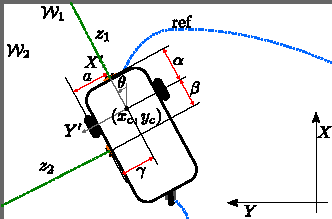
\includegraphics[scale=1.8]{figures/illustration_kalman.pdf}
\caption{Schematic overview of the robot moving in the world and measuring the distance to the walls. $(x_{\mathrm{c}},y_{\mathrm{c}})$ are the coordinates of the robot's center in the world coordinate system $XY$. The robot's orientation is determined by $\theta$, the angle between the $X$-axis and the robot's longitudinal axis $X'$. The dimensions $a$ and $\alpha,\beta,\gamma$ are to be measured for the state equations and output equations respectively.}
\label{fig:cartkalman}
\end{figure}

\paragraph{Step 1: Modeling the system}
Before designing an estimator, you need to model the system. Two equations should be derived:
\begin{enumerate}
    \item State equation $\mathbf{\dot{x}} = f(\mathbf{x}, \mathbf{u})$: The input of the system can be chosen as $\mathbf{u} = \begin{bmatrix}v\\ \omega\end{bmatrix}$, where $\omega$ [rad/s] denotes the rotational velocity of the robot around its center point, and $v$ [m/s] is the robot's forward translational velocity (i.e. along its longitudinal axis).
    \textit{What are the states $\mathbf{x}$ of the system? What is the relationship between state derivative $\mathbf{\dot{x}}$ and the state $\mathbf{x}$ and input $\mathbf{u}$?}
    \item Output equation $\mathbf{z} = h(\mathbf{x})$: The infrared sensors measure the distance to two separate walls (each sensor looks at a different wall).
    Assume a wall is given by $\mathcal{W} = \{(x,y) \,|\, ax+by=c\}$, after correcting the infrared measurements such that they measure the distance from the center of the cart, the ouput $\mathbf{z}$ is given by $\mathbf{z} = \mathrm{dist}((x_\mathrm{c},y_\mathrm{c}), \mathcal{W})$. \textit{Determine the corresponding output equation. That is, compute $\mathbf{z}$ as a function of $\mathbf{x}$.}
\end{enumerate}
Besides the state and output equation, two sources of noise are incorporated in the model.
\begin{enumerate}
    \item Process noise $\mathbf{w}$: this noise is added to the state equation and is assumed to have a normal distribution with zero mean and a diagonal covariance matrix $Q$. \textit{What are potential sources of process noise?}
    \item Measurement noise $\mathbf{v}$: this noise is added to the output equation and is assumed to have a normal distribution with zero mean and a diagonal covariance matrix $R$.
\end{enumerate}
Before you can implement a Kalman filter, you should discretize your state and output equation. Therefore you can use a forward Euler method ($\mathbf{\dot{x}} \approx \frac{\mathbf{x}_{k+1}-\mathbf{x}_k}{T_s}$). \textit{Discretize the system, such that you retrieve a model written as}
\begin{equation}
\label{modelequations}
\begin{aligned}
    \mathbf{x}_{k+1} &= f(\mathbf{x}_k, \mathbf{u}_k) + \mathbf{w}_k\,,\\
    \mathbf{z}_{k} &= h(\mathbf{x}_k) + \mathbf{v}_k\,.
\end{aligned}
\end{equation}

\paragraph{Step 2: Design of an extended Kalman filter}
As you should have noticed, the acquired system equations are non-linear. This implies that an \textit{extended} Kalman filter should be used as state estimator. \textit{Write down all steps of an update of the Kalman filter. Write down all involved equations.}

\paragraph{Step 3: Validate the Kalman filter in simulation}
Perform a simulation of the system in Matlab. In order to simulate the behavior of the cart, use the state and output equations \eqref{modelequations} and deliberately add process and measurement noise (with normal distribution and covariance matrix $Q$ and $R$). Implement the extended Kalman filter (do not deliberately add noise in its steps!) and apply a certain input trajectory. \textit{Monitor the estimated position and orientation $(\hat{x}_c, \hat{y}_c, \hat{\theta}_c)$ and monitor its convergence. For the position this can be done by plotting the confidence ellipsoids on its estimated position in the $XY$ plane. What happens when you leave out the correction step (dead-reckoning)? What happens when your modeled noise (by means of $Q$ and $R$) does not agree with the simulated noise? What happens when you only have one infrared sensor and one wall to look at?}

\paragraph{Step 4: Validate the Kalman filter in practice}
Implement the extended Kalman filter on the Arduino and perform similar experiments as in step 3. As the infrared sensors are fixed rigidly to the cart's frame and as they have a maximum range of 30cm, it is possible that they lose track of their corresponding wall. \textit{Find a way of discarding an infrared measurement when it becomes invalid.} As it is very hard to model the process and measurement noise acting on the system, the corresponding covariance matrices $Q$ and $R$ should be tuned in practice. \textit{Analyze and explain what happens if you change the covariance matrices.}

\paragraph{Step 5: Design of a state feedback controller}
Since you now have an estimate of the cart's position and orientation, you can close the loop and implement a state feedback controller to follow a certain position and orientation trajectory. This controller takes as input the tracking error
\begin{equation}
    \mathbf{\hat{e}_x} = \mathbf{x}_{\mathrm{ref}} - \mathbf{\hat{x}} %
                      = \begin{bmatrix} x_{\mathrm{c,ref}} - \hat{x}_{\mathrm{c}} \\ y_{\mathrm{c,ref}} - \hat{y}_{\mathrm{c}}  \\ \theta_{\mathrm{ref}} -\hat{\theta}\end{bmatrix}\,.
\end{equation}
The control law then corresponds to the static relation between $\mathbf{u}$ and $\mathbf{\hat{e}_x}$. As the system-to-control is non-linear and only design approaches for linear systems were addressed during the course, a heuristic control approach is used to design the state feedback controller. The control law is computed by first expressing the state error in the coordinate system $X'Y'$ attached to the cart (see Figure \ref{fig:cartkalman}). \textit{Determine the rotation matrix that is required for the conversion of $(x,y,\theta)$, expressed in the world coordinate system $XY$, to $(x',y',\theta')$, expressed in the local coordinate system $X'Y'$. As this conversion depends on the orientation $\theta$ of the cart, use the estimate $\hat{\theta}$ to convert $\mathbf{\hat{e}_x}$ to $\mathbf{\hat{e}_x}'$}.
A static feedback gain $\mathbf{K}$ is proposed to compute $\mathbf{u}$ from $\mathbf{\hat{e}_x}'$ ($\mathbf{u} = \mathbf{K} \mathbf{\hat{e}_x}'$) with the following structure:
\begin{equation}
\mathbf{K} = \begin{bmatrix} k_x & 0 & 0 \\ 0 & k_y & k_\theta \end{bmatrix}\,
\end{equation}
\textit{Can you explain this structure? Extend your simulation and code on the Arduino with this feedback law. Implement a reference trajectory. As the cart has only two control signals not all reference trajectories $(x_{\mathrm{c,ref}},y_{\mathrm{c,ref}},\theta_{\mathrm{ref}})$ are feasible. How to construct feasible trajectories, other than a straight line? Analyze the effect of the gains $k_x$, $k_y$, $k_\theta$ and tune them to get a proper tracking controller. Improve the tracking performance by adding an explicit feedforward signal to the system input:
\begin{equation}
\mathbf{u} = \mathbf{u}_{FF} + \mathbf{K}\mathbf{\hat{e}_x}'
\end{equation}
Determine $\mathbf{u}_{FF}$ from the reference trajectory $(x_{\mathrm{c,ref}},y_{\mathrm{c,ref}},\theta_{\mathrm{ref}})$. Don't you have this information already by composing this reference trajectory?}.

\end{document}
